\documentclass{article}

% use for selecting Dutch as language
\usepackage[dutch]{babel}

% Used to break lines eagerly, to not overflow them into the column to the right of it
\sloppy

% Use font Spartan
\usepackage{fontspec}
\setmainfont{Spartan}[
    Path=./font/,
    Scale=0.9,
    Extension = .ttf,
    UprightFont=*-Regular,
    BoldFont=*-ExtraBold,
    ItalicFont=*-Regular, % Italic not downloaded...
    BoldItalicFont=*-ExtraBold % BoldItalic not downloaded...
]

% Used for multi columns, and black line indicator
\usepackage{paracol}
\columnratio{0.35}
\usepackage{color}
\setlength{\columnseprule}{0.4pt}
\setlength{\columnsep}{4em}
\def\columnseprulecolor{\color{black}}

% Move the line separator more to the right (80% and 20%)
\usepackage{lipsum}
\usepackage{xpatch}
\makeatletter
\xpatchcmd{\pcol@hfil}{.5}{.8}{}{}
\xpatchcmd{\pcol@hfil}{.5}{.8}{}{}
\xpatchcmd{\pcol@hfil}{.5}{.2}{}{}
\xpatchcmd{\pcol@hfil}{.5}{.2}{}{}
\makeatother

% For using color in tables, and Y as centered column in tabularX
\usepackage[table]{xcolor}
\usepackage{tabularx}
\newcolumntype{Y}{>{\centering\arraybackslash}X}

% Used for page margins
\usepackage{geometry}
\geometry{
    a4paper,
    total={170mm,257mm},
    left=20mm,
    top=20mm,
}

% Section titles formatting
\usepackage{setspace}
\usepackage{titlesec}
\titleformat{\section}[block]{\Large\bfseries\filcenter}{}{1em}{}
\newcommand{\sectionfont}{\Large\bfseries\filcenter\uppercase}
\titleformat{\subsection}
    {\titlerule     
     \vspace{1.1em} % padding top
     \sectionfont}
    {\thesection}{1em}
    {\sectionfont}[\vspace{0.6em}\titlerule] % padding bottom
\titlespacing*{\subsection}
    {0pt} % margin left
    {1.5em} % margin top
    {0pt} % margin bottom

% No numbers in the Table of Contents
\setcounter{secnumdepth}{0}

% Smaller bullet points in first itemize level 
\renewcommand\labelitemi{\tiny$\bullet$}

% For changing margins in itemize
\usepackage{enumitem}
\setlist[itemize]{noitemsep, topsep=0pt}

% Remove indentation of first line of paragraph and after \newline
\setlength{\parindent}{0pt}

% For using images
\usepackage{graphicx}
\graphicspath{ {./voorgerechten/fotos}{./hoofdgerechten/fotos}{./nagerechten/fotos} }

% Foreach loops
\usepackage{pgffor}

% For using symbols
\usepackage{gensymb}





% Start of actual document
\title{Receptenboek}
\author{Aïsha Acda \and Mark Acda}

\date{Maart 2023}

\begin{document}

\maketitle

\tableofcontents

\newpage
\section{Voorgerechten}
% \newpage
\subsection{Naam van voorgerecht}

\newpage
\section{Hoofdgerechten}
% \newpage

\begin{center}
    \uppercase{Hoofdgerecht}
\end{center}
\rule{\linewidth}{0.4pt}
\subsection{Couscous familierecept}
\rule{\linewidth}{0.4pt}

\hspace{0.5cm}

\begin{paracol}{2}

\uppercase{\textbf{Ingrediënten}}

\hspace{0.25cm}

4-6 personen

\hspace{0.5cm}

\begin{itemize}
    \setlength\itemsep{0em}
    \item 2 uien
    \item 3 tenen knoflook
    \item Handje rozijnen
    \item 2-3 eieren
    \item 2 groentebouillonblokjes
    \item 1 winterpeen
    \item 1 knolselderij
    \item 1 courgette
    \item 1 (fles)pompoen
    \item Rozijnen
    \item Kikkererwten
    \item Tuinbonen
    \item Couscous
    \item +/- 1 kg kippenbouten of drumsticks
    \item 2 el olijfolie
    \item 2 tl kurkuma
    \item 2 tl gemalen koriander
    \item 1 tl komijnpoeder
    \item 1 tl karwijzaadpoeder
    \item 1 tl paprikapoeder
    \item \textonehalf tl gemberpoeder
    \item \textonehalf tl zwarte peper
\end{itemize}

\hspace{1cm}\newline
\uppercase{\textbf{Notities}}
\hspace{1cm}\newline
\begin{itemize}
    \setlength\itemsep{1em}
    \item In plaats van kip kan ook vlees gebruikt worden of niets (vega). \textbf{Het marineren hiervan kan de dag van tevoren al, maar het liefst een paar uur voor het maken van de couscous.}
    \item Met de groenten kan gevarieerd worden. Paprika is ook erg lekker, maar ook bosui erdoor.
\end{itemize}

\newpage % remove this when the images should start directly below 'Notities'

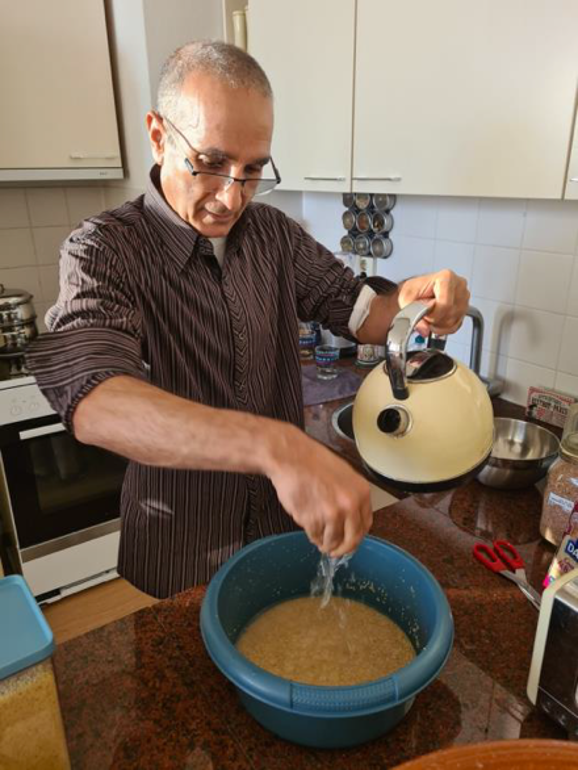
\includegraphics[width=\linewidth]{hoofdgerechten/fotos/couscous2.png}
\hspace{1cm}\newline
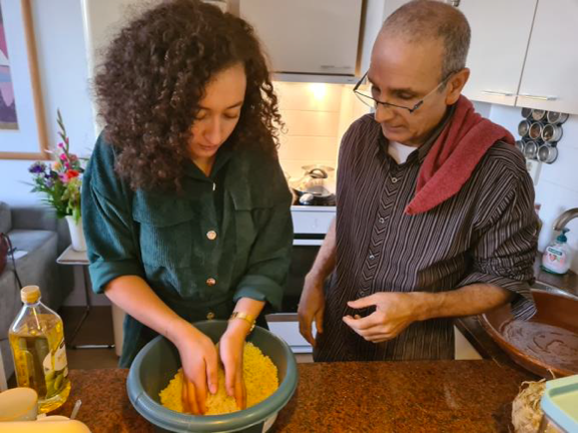
\includegraphics[width=\linewidth]{hoofdgerechten/fotos/couscous3.png}
\hspace{1cm}\newline
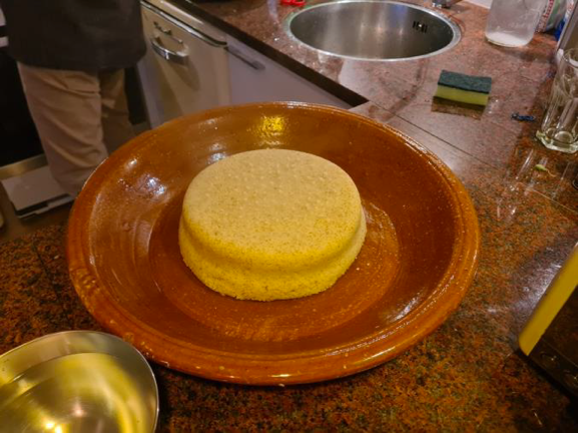
\includegraphics[width=\linewidth]{hoofdgerechten/fotos/couscous4.png}
\hspace{1cm}\newline
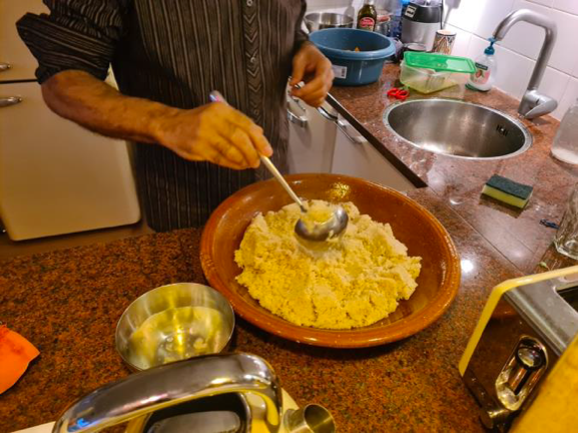
\includegraphics[width=\linewidth]{hoofdgerechten/fotos/couscous5.png}
\hspace{1cm}\newline

\vspace*{\fill}\switchcolumn

{\renewcommand{\arraystretch}{2}
    \begin{tabularx}{\linewidth}{YYY} % Y is custom column that is centered
        \rowcolor[RGB]{236, 234, 231}
         Voorbereiding: & Bereiding: & Totale tijd: \\ 
         10 min & 1 tot 2 uur & 2 uur \\
         \hline
    \end{tabularx}
}

\hspace{1cm}\newline

% TODO: crop bottom of picture to be x cm tall
% https://tex.stackexchange.com/questions/57418/crop-an-inserted-image
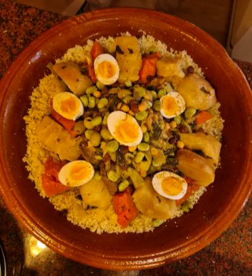
\includegraphics[width=\linewidth]{hoofdgerechten/fotos/couscous1.png}

\hspace{1cm}\newline

\uppercase{\textbf{Bereiden}}
\begin{enumerate}
    \item Snij eerst de uien in grove parten en snij/pers de knoflook fijn (dit gaan straks bij de gemarineerde kip).
    \item Begin nu met het marineren van de kip. Doe de kip in een schaal en doe hierbij de olijfolie en grote theelepels kurkuma, gemalen koriander, komijnpoeder, karwijzaadpoeder, paprikapoeder, gemberpoeder, zwarte peper en een snufje cayennepeper. Voeg ook de fijngesneden knoflook toe. Meng alles door elkaar en leg er vervolgens de ui parten bovenop. Dek af en zet in de koelkast.
    \item Meng alle kruiden in dezelfde hoeveelheden, maar dan kleine theelepels, in een apart klein schaaltje en bewaar dit voor later.
    \item Snij dan de groenten in grove stukken en bewaar voor later.
    \item Doe de couscous in een couscousschaal en giet er wat koud water over waardoor het net onder staat. Laat dit ongeveer 15 minuten intrekken. Maak vervolgens de couscous los.
    \item Breng water aan de kook in de onderste helft van de pan. Vul de bovenste helft van de pan met de couscous uit de couscousschaal en maak er wat gaten in tot de bodem met de achterkant van een pollepel. Als het water kookt zet je de couscous op de onderste helft van de pan en laat je deze 20 tot 30 minuten stomen.
    \item Haal na het stomen de couscous uit de pan en kiep deze om in de couscousschaal. Schep om met een lepel. Pak een kopje gekookt/heet water (kan ook uit de pan) en voeg hier een theelepeltje zout aan toe. Voeg dit vervolgens gelijkmatig toe aan de couscous in de couscousschaal en schep om. Voeg ook wat olijfolie toe en schep weer om. Laat afkoelen.
    \item Gooi ondertussen de onderste helft van de pan leeg. Leg hier vervolgens de gemarineerde kip met uien in en zet het vuur aan. Bak de kip 1 minuut. Voeg vervolgens water toe tot de kip bijna onder staat. Leg hier alvast de knolselderij en de pompoen bovenop en voeg wat meer water toe. Breng aan de kook.
    \item Doe de couscous uit de couscousschaal terug in de bovenste helft van de pan. Laat deze vervolgens weer 20 tot 30 minuten stomen boven de kip en de groenten.
    \item Haal de couscous uit de pan en kiep om in de couscousschaal. Schep om en laat afkoelen. Voeg eventueel wat olijfolie toe en maak los met je handen zodat zoveel mogelijk klontjes weg zijn.
    \item Voeg ondertussen het aparte schaaltje kruiden toe aan de kip en groenten in de pan. Kruimel hier ook de groentebouillonblokjes boven. Leg de stukken courgette en wortel erbij.
    \item Doe na 10 tot 15 minuten de couscous weer in de bovenste helft van de pan en laat deze weer 20 tot 30 minuten stomen boven de kip en de groenten.
    \item Ondertussen kun je beginnen met het koken van de eieren in een aparte pan of eierkoker. Zorg ervoor dat de eieren medium tot hard gekookt zijn.
    \item Haal de couscous uit de pan en kiep in de couscousschaal. Maak weer los met een lepel en je handen. Zorg ervoor dat de couscous gelijk over de schaal verdeeld is en maak de randen wat hoger met een kuiltje in het midden.
    \item Voeg een handje rozijnen, kikkererwten en tuinbonen toe aan de groenten en verwarm even mee.
    \item Nu kan de couscous opgebouwd worden. Begin met een stapeltje maken van de kip in het midden van de kuil in de schaal. Daaromheen leg je de groenten zodat de kip niet meer te zien is. Gooi hier overheen wat van de saus met kikkererwten, ui, tuinbonen en rozijnen. Je kunt ook wat saus over de couscous doen.
    \item Snij de eieren in de lente doormidden en verdeel over de schaal.
    \item Serveer de saus los in een bakje bij de couscous.
\end{enumerate}

\end{paracol}
 % TODO: remove this file couscous.txt
\begin{filecontents*}{recipeGenerator.py}

def addCurlyBraces(s):
    return "{" + s + "}"

class Recept:
    def __init__(self, titel, ingredienten, notities, voorbereiding, bereiding, totaleTijd, personen, stappen, afbeeldingen):
        self.titel = addCurlyBraces(titel)
        self.voorbereiding = addCurlyBraces(voorbereiding)
        self.bereiding = addCurlyBraces(bereiding)
        self.totaleTijd = addCurlyBraces(totaleTijd)
        self.personen = addCurlyBraces(personen)
        self.titelAfbeelding = afbeeldingen[0]
        
        self.ingredienten = ','.join(map(addCurlyBraces, ingredienten))
        self.notities = ','.join(map(addCurlyBraces, notities))
        self.stappen = ','.join(map(addCurlyBraces, stappen))
        self.afbeeldingen = ','.join(afbeeldingen[1:])
    
    def writeToTemplate(self):
        txt = open("template.tex", "r").read()
        txt = txt.replace("__titel__", self.titel)
        txt = txt.replace("__ingredienten__", self.ingredienten)
        txt = txt.replace("__notities__", self.notities)
        txt = txt.replace("__voorbereiding__", self.voorbereiding)
        txt = txt.replace("__bereiding__", self.bereiding)
        txt = txt.replace("__totaleTijd__", self.totaleTijd)
        txt = txt.replace("__personen__", self.personen)
        txt = txt.replace("__stappen__", self.stappen)
        txt = txt.replace("__titelAfbeelding__", self.titelAfbeelding)
        txt = txt.replace("__afbeeldingen__", self.afbeeldingen)
        return txt

recepten = [
    Recept(
	"Couscous familierecept",
	[
		"2 uien",
		"3 tenen knoflook",
		"2-3 eieren",
		"2 groentebouillonblokjes",
		"1 winterpeen",
		"1 knolselderij",
		"1 courgette",
		"1 (fles)pompoen",
		"rozijnen",
		"kikkererwten",
		"tuinbonen",
		"couscous",
		"+/- 1 kg kippenbouten of drumsticks",
		"2 el olijfolie",
		"2 tl kurkuma",
		"2 tl gemalen koriander",
		"1 tl komijnpoeder",
		"1 tl karwijzaadpoeder",
		"1 tl paprikapoeder",
		"1/2 tl gemberpoeder",
		"1/2 tl zwarte peper"
	],
	[
		"In plaats van kip kan ook vlees gebruikt worden of niets (vega). Het marineren hiervan kan de dag van tevoren al, maar het liefst een paar uur voor het maken van de couscous.",
		"Met de groenten kan gevarieerd worden. Paprika is ook erg lekker, maar ook bosui erdoor."
	],
	"10 min",
	"1 tot 2 uur",
	"2 uur",
	"4 - 6 personen",
	[
		"Snij eerst de uien in grove parten en snij/pers de knoflook fijn (dit gaan straks bij de gemarineerde kip).",
		"Begin nu met het marineren van de kip. Doe de kip in een schaal en doe hierbij de olijfolie en grote theelepels kurkuma, gemalen koriander, komijnpoeder, karwijzaadpoeder, paprikapoeder, gemberpoeder, zwarte peper en een snufje cayennepeper. Voeg ook de fijngesneden knoflook toe. Meng alles door elkaar en leg er vervolgens de ui parten bovenop. Dek af en zet in de koelkast.",
		"Meng alle kruiden in dezelfde hoeveelheden, maar dan kleine theelepels, in een apart klein schaaltje en bewaar dit voor later.",
		"Snij dan de groenten in grove stukken en bewaar voor later.",
		"Doe de couscous in een couscousschaal en giet er wat koud water over waardoor het net onder staat. Laat dit ongeveer 15 minuten intrekken. Maak vervolgens de couscous los.",
		"Breng water aan de kook in de onderste helft van de pan. Vul de bovenste helft van de pan met de couscous uit de couscousschaal en maak er wat gaten in tot de bodem met de achterkant van een pollepel. Als het water kookt zet je de couscous op de onderste helft van de pan en laat je deze 20 tot 30 minuten stomen.",
		"Haal na het stomen de couscous uit de pan en kiep deze om in de couscousschaal. Schep om met een lepel. Pak een kopje gekookt/heet water (kan ook uit de pan) en voeg hier een theelepeltje zout aan toe. Voeg dit vervolgens gelijkmatig toe aan de couscous in de couscousschaal en schep om. Voeg ook wat olijfolie toe en schep weer om. Laat afkoelen.",
		"Gooi ondertussen de onderste helft van de pan leeg. Leg hier vervolgens de gemarineerde kip met uien in en zet het vuur aan. Bak de kip 1 minuut. Voeg vervolgens water toe tot de kip bijna onder staat. Leg hier alvast de knolselderij en de pompoen bovenop en voeg wat meer water toe. Breng aan de kook.",
		"Doe de couscous uit de couscousschaal terug in de bovenste helft van de pan. Laat deze vervolgens weer 20 tot 30 minuten stomen boven de kip en de groenten.",
		"Haal de couscous uit de pan en kiep om in de couscousschaal. Schep om en laat afkoelen. Voeg eventueel wat olijfolie toe en maak los met je handen zodat zoveel mogelijk klontjes weg zijn.",
		"Voeg ondertussen het aparte schaaltje kruiden toe aan de kip en groenten in de pan. Kruimel hier ook de groentebouillonblokjes boven. Leg de stukken courgette en wortel erbij.",
		"Doe na 10 tot 15 minuten de couscous weer in de bovenste helft van de pan en laat deze weer 20 tot 30 minuten stomen boven de kip en de groenten.",
		"Ondertussen kun je beginnen met het koken van de eieren in een aparte pan of eierkoker. Zorg ervoor dat de eieren medium tot hard gekookt zijn.",
		"Haal de couscous uit de pan en kiep in de couscousschaal. Maak weer los met een lepel en je handen. Zorg ervoor dat de couscous gelijk over de schaal verdeeld is en maak de randen wat hoger met een kuiltje in het midden.",
		"Voeg een handje rozijnen, kikkererwten en tuinbonen toe aan de groenten en verwarm even mee.",
		"Nu kan de couscous opgebouwd worden. Begin met een stapeltje maken van de kip in het midden van de kuil in de schaal. Daaromheen leg je de groenten zodat de kip niet meer te zien is. Gooi hier overheen wat van de saus met kikkererwten, ui, tuinbonen en rozijnen. Je kunt ook wat saus over de couscous doen.",
		"Snij de eieren in de lente doormidden en verdeel over de schaal.",
		"Serveer de saus los in een bakje bij de couscous."
	],
	[
		"couscous1",
		"couscous2",
		"couscous3",
		"couscous4",
		"couscous5"
	]
),
Recept(
	"Traditioneel stoofvlees",
	[
		"750 g rib- of sukadelappen",
		"300 ml water",
		"2 uien (gesnipperd)",
		"2 plakjes ontbijtkoek",
		"1 1/2 runderbouillonblokje",
		"4 laurierblaadjes",
		"3 kruidnagels",
		"4 eetlepels azijn",
		"roomboter",
		"paprikapoeder",
		"cayennepeper",
		"peper \& zout"
	],
	[
		"Voor 4 personen is dit net iets te weinig vlees"
	],
	"15 min",
	"4 uur",
	"4 uur 15 minuten",
	"4 personen",
	[
		"Haal het vlees ongeveer een half uur voor je gaat beginnen uit de koelkast en laat het op kamertemperatuur komen.",
		"Strooi peper, zout, paprikapoeder en cayennepeper aan beide kanten van het vlees.",
		"Doe ruim roomboter in een braadpan en bak hierin het vlees om en om aan voor een paar minuten tot het goudbruin is. Haal het vlees uit de pan en leg het even apart.",
		"Fruit de uien even aan in de braadpan en voeg eventueel nog een beetje extra roomboter toe.",
		"Als de ui glazig begint te worden voeg je 300 ml water, 1½ runderbouillonblokje, 4 el azijn, 3 laurierblaadjes en 3 kruidnagels toe.",
		"Breng dit alles rustig roerend aan de kook en als het kookt doe je het vlees erbij. Leg de plakjes ontbijtkoek erop. Breng het geheel weer aan de kook, doe de deksel op de pan en zet het vuur laag.",
		"Laat dit voor minimaal 3 of 4 uur opstaan (af en toe even kijken, vlees omdraaien en als het droog wordt kun je wat water toevoegen). Heb je de tijd, laat het dan langer opstaan, des te langer, des te lekkerder het vlees wordt. Een uur of 6 is hierbij een mooi uitgangspunt. Wil je serveren en zit er nog te veel vocht in de pan, haal dan even de deksel eraf en laat het even inkoken."
	],
	[
		"stoofvlees1"
	]
),
Recept(
	"Lasagne",
	[
		"2 uien",
		"2 tenen knoflook",
		"300 g gehakt",
		"2 paprika's",
		"1 courgette",
		"3 tomaten",
		"600 g tomatensaus",
		"lasagnebladen",
		"1 bol mozzarella",
		"150 g geraspte kaas",
		"Italiaanse kruiden",
		"peper \& zout"
	],
	[
		"Als tomatensaus kun je gewone pastasaus gebruiken.",
		"Erg lekker met een caprese salade ernaast.",
		"Het gehakt kan ook vervangen wroden door vegetarische rulstukjes.",
		"Je kunt de lasagne 2-3 dagen bewaren in de koelkast."
	],
	"30 min",
	"44 min",
	"1 uur 15 minuten",
	"4 personen",
	[
		"Verwarm de oven voor op 200\degree C.",
		"Snipper de uien en pers de teentjes knoflook uit, fruit dit aan in een pan met een beetje olie. Voeg het gehakt toe en bak dit rul. Breng het gehakt op smaak met peper, zout en Italiaanse kruiden.",
		"Tijd om de ovenschaal te vullen: saus, bladen, saus, mozzarella, bladen, saus, bladen, saus en als laatste de geraspte kaas.",
		"Zet de lasagne 45 minuten in de oven op 200\degree C (boven- en onderwarmte)."
	],
	[
		"lasagne1"
	]
),
Recept(
	"Korkante kip pokébowl",
	[
		"500 g sushirijst",
		"4 el azijn",
		"4 tl suiker",
		"4 kipschnitzels (krokant)",
		"1 mango",
		"10 radijsjes",
		"komkommer",
		"100 g edamame",
		"kiemgroenten",
		"sesamzaadjes",
		"6 el mayonaise of yogonaise",
		"1 el sriracha"
	],
	[
		"Er zijn veel variaties te maken op deze poké bowl. Je kunt bijvoorbeeld avocado toevoegen of peen julienne."
	],
	"15 min",
	"15 min",
	"30 minuten",
	"4 personen",
	[
		"Laat de sushirijst eerst een kwartier wellen in koud water.",
		"Spoel het vervolgens om en doe het water erbij volgens de verpakking.",
		"Breng de rijst aan de kook, zet het vuur laag en kook het in ongeveer 10 tot 15 minuten met de deksel op de pan gaar.",
		"In een kommetje meng je de azijn met de suiker goed door elkaar.",
		"Dit mengsel schep je vervolgens door de sushirijst wanneer deze gaar is. Laat de sushirijst daarna volledig afkoelen.",
		"Bak de kipschnitzels volgens de verpakking in een pan.",
		"Maak ondertussen de saus door de mayonaise, chilisaus en eventueel wat gembersiroop te mengen.",
		"Snij de komkommer in stukjes en de mango en radijs in plakjes.",
		"Verdeel de afgekoelde sushirijst over 2 kommen, snij de krokante kipfilet in repen en verdeel over de kommen samen met de groenten. Verdeel naar smaak de saus over de kip en garneer met sesamzaadjes."
	],
	[
		"pokebowl1"
	]
),
Recept(
	"Chipolata baketray",
	[
		"1.2 kg (ovengroente) zoete aardappel, rode paprika en broccoli",
		"165 g groene olijven met knoflook",
		"8 runderchipolata",
		"3 el milde harissa",
		"2 el milde olijfolie",
		"1 mespunt zout",
		"250 g tomaatjes"
	],
	[],
	"10 min",
	"30 min",
	"40 minuten",
	"4 personen",
	[
		"Verwarm de oven voor op 200\degree C.",
		"Verdeel de ovengroente over een met bakpapier beklede bakplaat. Verdeel de olijven erover.",
		"Snijd de runderchipolata elk in 3 stukken en meng de worstjes met de harissa in een kom. Laat staan tot gebruik. Besprenkel ondertussen de groenten met de olie en bestrooi met zout. Leg er de tomaatjes tussen. Rooster 25-30 minuten. In het midden van de oven tot alles goudbruin en gaar is. Schep halverwege om en leg de worstjes erbij."
	],
	[
		"chipolata1"
	]
),
Recept(
	"Plaatpizza tomaatjes",
	[
		"550 g koelvers pizzadeeg (spelt/volkoren)",
		"70 g pesto arrabiata",
		"250 g mozzarella",
		"500 g snoepgroente tomatenmix",
		"3 el kappertjes in pot",
		"40 g rucola"
	],
	[],
	"10 min",
	"20 min",
	"30 minuten",
	"4 personen",
	[
		"Verwarm de oven voor op 200\degree C.",
		"Rol het pizzadeeg met het bakpapier uit op de bakplaat. Bestrijk het pizzadeeg met de pesto.",
		"Snijd de mozzarella in blokjes van circa 1 cm en halveer de snoeptomaatjes. Verdeel eerst de mozzarella en vervolgens de snoeptomaatjes over het deeg. Bestrooi met de kappertjes. Bak in 18-20 minuten. Goudbruin en krokant in de oven.",
		"Neem de gebakken pizza uit de oven en verdeel de rucola erover."
	],
	[
		"plaatpizza1"
	]
),
Recept(
	"Berber omelet/Tajine kefta",
	[
		"250 g gehakt",
		"1 tl zout",
		"1 tl zwarte peper",
		"1 tl kurkuma",
		"1 tl paprikapoeder",
		"1/2 tl gember",
		"1/2 tl komijn",
		"2 tenen knoflook",
		"4 tomaten",
		"2 el tomatenpuree",
		"1 grote ui",
		"olijven",
		"peterselie/koriander",
		"2-3 eieren",
		"brood"
	],
	[
		"Er zijn veel variaties mogelijk. Paprika of aardappel kan ook toegevoed worden.",
		"Kan ook geserveerd worden met friet."
	],
	"15 min",
	"45 min",
	"1 uur",
	"2-3 personen",
	[
		"Rasp de ui en de tomaten (of snij ze fijn). Voeg een klein beetje ui toe aan het gehakt.",
		"Meng alle kruiden en verdeel in tweeën. Meng het gehakt met de ene helft van de kruiden. Maak hiervan kleine balletjes en bak deze aan in een pan of tajine met olijfolie.",
		"Voeg de ui, knoflook en de tomaten toe. Dan de rest van de kruiden erbij en even laten pruttelen.",
		"Doe de tomatenpuree erbij en meng alles goed. Bak even op hoog vuur. Voeg dan een glas water toe (ongeveer 200 ml) en breng aan de kook. Laat op zacht vuur 45 minuten stoven met deksel tot het een mooi sausje is",
		"Verwarm de olijven mee en breek er de eieren boven en laat die stollen. Serveer met brood."
	],
	[
		"berber1"
	]
),
Recept(
	"Vegetarische risotto",
	[
		"2 el olijfolie",
		"300 g risottorijst",
		"1 el paprikapoeder",
		"900 g diepvries groenten (gegrild)",
		"330 ml tomato frito",
		"1 groentebouillonblokje",
		"650 ml water",
		"zwarte olijven (schijfjes)",
		"peper \& zout"
	],
	[],
	"5 min",
	"30 min",
	"35 min",
	"4 personen",
	[
		"Verhit de olie in een hapjespan en bak de rijst al omscheppend 2 minuten op middelhoog vuur.",
		"Voeg de paprikapoeder, diepvriesgroenten, tomato frito, groentebouillonblokje en het water toe en breng aan de kook.",
		"Laat zonder deksel op de pan 25 minuten zachtjes koken tot de rijst gaar is. Schep af en toe om.",
		"Voeg peper en zout toe en verwarm de olijven mee."
	],
	[
		"risotto1"
	]
),
Recept(
	"Pindasoep",
	[
		"2 tenen knoflook",
		"3 el wokolie",
		"400 g Chinese groentemix",
		"3 kippenbouillonblokjes",
		"300 g kipfiletblokjes",
		"1.3 l water",
		"100 g pindakaas",
		"2 el ketjap manis",
		"1 zakje kroepoek",
		"1-2 el sambal (optioneel)"
	],
	[],
	"5 min",
	"20 min",
	"25 min",
	"4 personen",
	[
		"Snijd de knoflook fijn. Verhit in een soeppan de olie. Fruit de groentemix en de knoflook circa 3 minuten.",
		"Voeg de kippenbouillonblokjes, kipblokjes en water toe, breng aan de kook en laat circa 5 minuten koken. Roer de pindakaas en de ketjap door de soep en verwarm circa 2 minuten mee. Voeg voor een pittigere soep 1 el sambal toe. Serveer de soep met kroepoek."
	],
	[
		"pinda1"
	]
),
Recept(
	"Italiaanse bonensalade",
	[
		"200 g borlotti bonen",
		"200 g cannellini bonen",
		"1 rode ui",
		"10 tomaatjes",
		"2 handjes rucola",
		"10 groene olijven",
		"1/2 komkommer",
		"sap van 1/2 citroen",
		"6 el olijfolie"
	],
	[
		"Heerlijke frisse zomerse salade!"
	],
	"20 min",
	"5 min",
	"25 min",
	"4 personen",
	[
		"Giet de bonen (uit blik) af in een vergiet en spoel even na met koud water",
		"Schil de ui en snij deze heel fijn. Halveer de tomaatjes en snij daarna in kwarten.",
		"Snij de komkommer doormidden en verwijder de zaadjes. Snij er daarna plakjes van.",
		"Meng het sap van de citroen met de olijfolie.",
		"Doe de bonen samen met de ui, tomaatjes, olijven, komkomeer in een schaal en hussel goed door. Voeg dan de rucola toe en schep nog een keer door elkaar.",
		"Schenk de dressing van citroensap en olijfolie over de Italiaanse bonensalade."
	],
	[
		"salade1"
	]
),
Recept(
	"Nacho schotel crispy chicken",
	[
		"500 g kipfilet",
		"1 zakje Santa Maria Crispy Chicken",
		"1 guacamolepakket",
		"200 g tortillachips",
		"400 g mexicaanse melange (blik bonduelle)",
		"75 g geraspte kaas",
		"1 el olijfolie",
		"verse koriander"
	],
	[
		"Dit gerecht kan zowel als hoofd-en borrelgerecht geserveerd worden."
	],
	"15 min",
	"10 min",
	"25 min",
	"4 personen",
	[
		"Verwarm de oven voor op 225\degree C.",
		"Snijd de kip in stukjes van circa 2 centimeter. Voeg de olie en de inhoud van het zakje Crispy Chicken Mix toe. Bedek alle stukjes goed met het mengsel.",
		"Leg de stukjes in een ingevette ovenschaal en zet in de oven voor circa 10 minuten.",
		"Volg de aanwijzingen op het guacamolepakket voor een heerlijke verse dip. Giet het vocht af van de Bonduelle groentenmelange.",
		"Doe de tortillachips in een ovenschaal en meng met de groentemelange. Haal de kip uit de oven en voeg toe aan de tortilla's. Bestrooi met kaas en zet kort in de oven tot de kaas mooi is gesmolten.",
		"Serveer met guacamole en verse koriander."
	],
	[
	"fotonogmaken",
	]
),
Recept(
	"Loempia Bowl",
	[
		"300 g peen julienne",
		"2 preien",
		"200 g taugé",
		"200 g glasnoedels",
		"500 g kipgehakt",
		"6 el sojasaus",
		"3 el gembersiroop",
		"2 tenen knoflook",
		"2 uien",
		"zwarte peper",
		"olijfolie"
	],
	[
		"Lekker met nog een fijngesneden bosui en wat fijngehakte cashewnoten/gebakken uitjes.",
		"Bij weinig tijd kun je ook een zak Oosterse roerbakgroenten gebruiken.",
		"Je kunt dit recept ook gebruiken als vulling voor loempia's van filodeeg bijvoorbeeld. Smeer het filodeeg in met olie en vouw dubbel, leg het mengel erin en rol op met de zijkanten naar binnen. Bestrijk de buitenkanten met olie en bak af in de oven op 180\degree C voor ongeveer 15 minuten. Draai af en toe om."
	],
	"10 min",
	"10 min",
	"20 minuten",
	"4 personen",
	[
		"Bereid de glasnoedels volgens de instructies op het pak.",
		"Snipper de ui en snijd de knoflook fijn. Maak de prei schoon en snijd in stukjes.",
		"Giet een scheutje olie in een (wok)pan en bak de ui en knoflook. Voeg na 2-3 minuten het kipgehakt en een snufje zwarte peper toe. Bak het gehakt rul. Daarka kan de peen julienne, prei, gembersiroop en sojasaus erbij.",
		"Bak dit 3 minuten en voeg dan de taugé en de gekookte glasnoedels toe. Meng alles door elkaar en zet na 1 minuut het vuur uit."
	],
	[
		"loempia1"
	]
),
Recept(
	"Hete kip",
	[
		"300 g witte rijst",
		"500 g kipfilet",
		"100 ml ketjap manis",
		"50 ml ketchup",
		"200 ml water",
		"3 1/2 el pindakaas",
		"1-2 el sambal",
		"peper \& zout",
		"kroepoek"
	],
	[
		"Lekker met komkommersalade ernaast of met groenten zoals prei en paprika erdoor."
	],
	"5 min",
	"30 min",
	"35 min",
	"4 personen",
	[
		"Kook de rijst volgens de aanwijzingen op de verpakking gaar.",
		"Snijd de kipfilet in reepjes. Breng de kip op smaak met (versgemalen) peper en zout. Verhit de olie in een braadpan en bak de kipreepjes goudbruin. Voeg de ketjap, ketchup en het water toe en breng aan de kook. Draai het vuur laag en stoof de kip 15 minuten.",
		"Roer de pindakaas erdoor, tot een dikke saus ontstaat. Breng de kip pittig op smaak met de sambal en voeg het zout toe. Laat de kip nog 5 minuten zachtjes stoven. Serveer de hete kip met de rijst en kroepoek."
	],
	[
	"hetekip1",
	]
),
Recept(
	"Ratatouille door studenten",
	[
		"1 courgette",
		"1 aubergine",
		"1 of 2 paprika's",
		"1 ui"
		"400 g tomatenblokjes in blik",
		"provençaalse kruiden (gedroogd)",
		"feta",
		"300 g rijst of couscous",
		"olijven",
		"peper \& zout"
	],
	[
		"Signature dish van Alice, Nienke en Aïsha."
	],
	"10 min",
	"10 min",
	"20 min",
	"4 personen",
	[
		"Kook de rijst of couscous volgens de aanwijzingen op de verpakking gaar.",
		"Snijd de courgette, aubergine, paprika en eventueel ui in blokjes. Verhit wat olie in een hapjes pan en bak de groenten vervolgens een paar minuten.",
		"Voeg de tomatenblokjes, provençaalse kruiden en wat peper en zout toe en verwarm nog 5 minuten door.",
		"Serveer de ratatouille met de rijst of couscous en garneer met wat verkruimelde feta en olijven."
	],
	[
	"ratatouille1",
	]
),
Recept(
	"Wraps met vissticks",
	[
		"2 el olijfolie",
		"15 diepvries vissticks",
		"400 g zwarte bonen in blik",
		"125 ml sour cream",
		"300 g gesneden rodekool",
		"1 avocado",
		"3 el jalapeñopepers in pot",
		"7.5 g verse koriander",
		"6 tortillawraps",
		"zwarte peper"
	],
	[],
	"5 min",
	"15 min",
	"20 min",
	"2 personen",
	[
		"Verhit de olie in een koekenpan en bak de vissticks op middelhoog vuur in 8 minuten goudgeel en gaar. Keer halverwege.",
		"Doe ondertussen de bonen in een vergiet, spoel af onder koud stromend water en laat uitlekken. Meng de sour cream met de rodekool en breng op smaak met versgemalen peper.",
		"Prak de zwarte bonen met een vork tot een grove puree. Breng op smaak met versgemalen peper. Halveer de avocado overlangs, verwijder de pit, schep het vruchtvlees met een lepel uit de schil en snijd in plakjes. Snijd de jalapeño grof en de koriander fijn.",
		"Verhit een koekenpan zonder olie of boter en verwarm de tortilla’s 20 seconden op middelhoog vuur. Beleg elke tortilla met rodekoolsalade, bonenpuree, wat plakjes avocado, vissticks en jalapeño. Bestrooi met wat koriander."
	],
	[
	"visstick1",
	]
),
Recept(
	"Herfstgroenten eenpanspasta",
	[
		"1 winterpeen",
		"1 ui",
		"20 g verse Italiaanse kruidenmix",
		"2 el olijfolie",
		"400 g koelverse muskaatpompoenstukjes",
		"250 g crème fraîche",
		"1 groentebouillonblokje",
		"300 g pasta",
		"400 ml water",
		"75 g Parmezaanse kaas",
		"peper \& zout"
	],
	[],
	"10 min",
	"20 min",
	"30 min",
	"4 personen",
	[
		"Halveer de peen in de lengte en snijd in plakjes van een 1/2 cm dik. Snijd de ui in dunne halve ringen. Ris de blaadjes van de takjes tijm en de takjes oregano uit het bakje Italiaanse kruidenmix en snijd de salieblaadjes uit het bakje fijn.",
		"Verhit de olie in een hapjespan en fruit de ui 3 minuten op middelhoog vuur. Voeg de fijngesneden kruiden, peen en pompoenstukjes toe en bak 2 minuten mee. Voeg de crème fraîche, het bouillonblokje, de ongekookte pasta en het water toe en roer goed door. Breng aan de kook en laat met de deksel op de pan 7 minuten zachtjes koken. Neem de deksel van de pan en laat nog 5 minuten koken. Roer regelmatig en breng op smaak met zout en peper.",
		"Rasp de Parmezaanse kaas met een fijne rasp. Verdeel de pasta over de borden en bestrooi met de Parmezaanse kaas."
	],
	[
	"eenpanspasta1",
	]
),
Recept(
	"Tjap tjoy",
	[
		"2 uien",
		"2 tenen knoflook",
		"250 g champignons",
		"1 rode paprika",
		"1 komkommer",
		"400 g minimaiskolfjes in blik",
		"3 el olijolie",
		"1 el sesamolie",
		"300 g kipfiletreepjes",
		"125 g taugé",
		"150 ml water",
		"1/2 kippenbouillonblokje",
		"1/2 el sambal",
		"1 el ketjap manis",
		"2 el maizena"
	],
	[
		"Lekker met rijst, nasi of bami."
	],
	"10 min",
	"10 min",
	"20 min",
	"4 personen",
	[
		"Snijd de uien in grote parten en haal de laagjes uit elkaar. Snijd de knoflook fijn. Snijd de champignons in plakjes en de paprika in reepjes. Snijd de komkommer in de lengte doormidden, verwijder de zaadlijsten en snijd het vruchtvlees en in schuine plakjes. Laat de minimais uitlekken.",
		"Verhit de zonnebloemolie en sesamolie in een wok en roerbak de ui 2 minuten op hoog vuur. Voeg de kipreepjes toe en roerbak 3 minuten mee. Voeg de knoflook, champignonplakjes en paprika toe en roerbak 3 minuten. Voeg de komkommer, minimais en taugé toe en roerbak nog 1 minuut",
		"Zet het vuur op laag. Voeg het water en de bouillonblokje toe en breng aan de kook. Meng ondertussen de sambal, oestersaus en ketjap met de maizena in een kommetje. Roer dit door het groentemengsel tot de bouillon begint te binden."
	],
	[
	"tjappie1",
	]
),
Recept(
	"Mexicaanse ovenschotel",
	[
		"500 g rundergehakt",
		"40 g burrito seasoningmix",
		"400 g tomatenblokjes in blik",
		"300 g mais in blik",
		"400 g chilibonen in blik",
		"100 g geraspte kaas",
		"150 g tortillachips",
		"1 rode puntparika"
	],
	[
		"Lekker met crème fraîche, guacamole/salsa dip en extra tortillachips ernaast."
	],
	"5 min",
	"30 min",
	"35 min",
	"4 personen",
	[
		"Verwarm de oven voor op 180\degree C.",
		"Verhit een koekenpan zonder olie of boter en bak het gehakt op middelhoog vuur in 5 minuten rul. Voeg de seasoningmix en tomatenblokjes toe en verwarm nog 2 minuten. Schep het mengsel in de ovenschaal.",
		"Laat de maïskorrels uitlekken en verdeel over het gehaktmengsel. Verdeel hier achtereenvolgens de chilibonen, de helft van de kaas, de helft van de tortillachips en de rest van de kaas over.",
		"Verwijder de steelaanzet en zaadlijsten van de paprika en snijd het vruchtvlees in ringen. Verdeel over de schotel. Bak de ovenschotel in het midden van de oven in circa 20 minuten goudbruin. Serveer met de rest van de tortillachips."
	],
	[
	"mexicaans",
	]
),
Recept(
	"Gevulde puntpaprika",
	[
		"300 g couscous",
		"400 ml kokend water",
		"1/2 groentebouillonblokje",
		"8 puntpaprika's"
		"2 uien/sjalotjes",
		"15 g verse munt",
		"150 g feta",
		"4 g paprikapoeder",
		"5 g komijnpoeder",
		"4 el olijfolie",
		"40 g gewelde abrikozenstukjes",
		"peper \& zout"
	],
	[
		"Lekker met veldsla."
	],
	"20 min",
	"15 min",
	"35 min",
	"4 personen",
	[
		"Verwarm de oven voor op 200\degree C. Los het halve bouillonblokje op in het kokende water. Doe de couscous in een kom en schenk er de bouillon over en roer door. Dek af en laat 10 minuten staan",
		"Halveer ondertussen de paprika’s in de lengte, verwijder de zaadlijsten maar laat de steeltjes zitten. Snipper de sjalotten, snijd de blaadjes van de munt fijn en verkruimel de feta.",
		"Roer de couscous los met een vork en meng de sjalot, paprikapoeder, komijn en olie erdoor. Schep de abrikozenstukjes, de helft van de munt en feta erdoor en breng op smaak met peper en eventueel zout.",
		"Verdeel de couscous over de paprikahelften en leg op een met bakpapier beklede bakplaat. Bak de paprika’s circa 15 minuten onder in de oven.",
		"Bestrooi met de rest van de munt en serveer."
	],
	[
	"paprika1",
	]
)
]

for recept in sorted(recepten, key=lambda x: x.titel):
     print(recept.writeToTemplate())

\end{filecontents*}

\input{|python recipeGenerator.py}

\newpage
\section{Salades}
% \newpage
\subsection{Naam van salade}

\newpage
\section{Nagerechten}
% \newpage
\subsection{Naam van nagerecht}

\end{document}
